\documentclass{article}
\usepackage{graphicx} 
\usepackage{float}
\usepackage{booktabs}
\usepackage{array}
\usepackage{arydshln}
\usepackage{siunitx}
\usepackage{hyperref}
\usepackage{cancel}
\usepackage{changepage}
\usepackage{placeins}
\usepackage{enumitem}
\usepackage{siunitx}
\usepackage{lipsum}
\usepackage[most]{tcolorbox}


%\usepackage{showframe}
\usepackage{times}

\DeclareSIUnit{\atm}{atm}

\usepackage{tabularx}
\usepackage{amsmath, amssymb, amscd, MnSymbol, mathrsfs}
\usepackage{cellspace}
\usepackage{tikz}
\usetikzlibrary{calc,3d, patterns, angles, quotes, decorations.markings, decorations.pathmorphing, hobby}
\usepackage{xfrac}

\usepackage{chemfig}
\usepackage{caption}
\usepackage{bm}
\usepackage{pdfpages}
\usepackage{empheq}
\usepackage{pgfplots}
\usepackage{pgfplotstable}
\usepackage{xstring}

\pgfplotsset{compat=1.18}
\usepackage[oldvoltagedirection]{circuitikz}
\usepackage{microtype}
\usepackage{tikz-3dplot}
\usepackage{textcomp}
% Custom commands
\newcommand{\vect}[1]{\boldsymbol{\mathbf{#1}}}
\newcolumntype{C}{>{\centering\arraybackslash}X}
\newcolumntype{M}[1]{>{\centering\arraybackslash}m{#1}}

%\usetikzlibrary{external}
%\tikzexternalize[prefix=figures/]

\newcommand\myfrac[2]{\sfrac{#1\mkern-1.2mu}{#2}}
\usepackage{xcolor}

% Define custom colors
\definecolor{darkblue}{rgb}{0.1,0.1,0.5} %  dark blue shade
\definecolor{formalshade}{rgb}{0.95,0.95,1} % light blue shade for the background

% For the adjustwidth environment
\PassOptionsToPackage{strict}{changepage}
\usepackage{changepage}

% For formal definitions
\usepackage{framed}

\newcommand{\formalsource}{} % Initialize an empty macro to store the source text

\newenvironment{formal}[3][]{% Start of the environment
	\renewcommand{\formalsource}{#1}% Store the optional argument
	\def\FrameCommand{%
		\hspace{1pt}%
		{\color{#2}\vrule width 2pt}%
		{\color{#3}\vrule width 4pt}%
		\colorbox{#3}%
	}%
	\MakeFramed{\advance\hsize-\width\FrameRestore}%
	\noindent\hspace{-4.55pt}% Disable indenting the first paragraph
	\begin{adjustwidth}{}{7pt}%
		\vspace{2pt}%
	}%
	{%
		\vspace{4pt}%
		\ifx\formalsource\empty % Check if the source is empty
		\else
		\hfill{\footnotesize{\formalsource}}% Align source to the bottom-right
		\fi
	\end{adjustwidth}\endMakeFramed%
}


% Custom itemize list with images for positive and negative items
\newlist{gitemize}{itemize}{1} % Just one level for the list
\setlist[gitemize,1]{
	leftmargin=2.8em, % Adjust the margin for the list
	labelsep=1em % Control the space between the label and the list item
}

% Define checkmark and cross symbols for positive and negative items
\newcommand{\checkitem}{\raisebox{-0.25\height}{\includegraphics[width=0.4cm]{checkmark.png}}}
\newcommand{\crossitem}{\raisebox{-0.25\height}{\includegraphics[width=0.4cm]{cross.png}}}


\usepackage[left=0.8in,right=0.8in,top=0.5in,bottom=0.69in,includeheadfoot,letterpaper]{geometry}
\usepackage{fancyhdr}
\usepackage{graphicx}
\usepackage{tabularray}
\usepackage{varwidth} 


\newcommand{\wm}[2]{%
	\begin{minipage}{#1\textwidth}
		\centering
		#2
	\end{minipage}%
}

\pagestyle{fancy}
\fancyhf{}


\renewcommand{\headrulewidth}{0.4pt}
\renewcommand{\footrulewidth}{0.4pt}

\fancyhead[L]{
\includegraphics[height=1.2cm]{images/Kingston_University_London_logo_200-tablet.png}}
\fancyhead[R]{EG4023 – ME – IMechE Design Challenge Project}
\fancyfoot[C]{Department of Mechanical Engineering}
\fancyfoot[R]{\thepage}

\usepackage{scalerel}
\usepackage{pythonhighlight}
\setlength{\headheight}{30pt}
\setlength{\footskip}{20pt}



\usepackage[export]{adjustbox}
\usepackage{tocloft}
\renewcommand{\cfttoctitlefont}{}
\renewcommand{\contentsname}{}
\renewcommand{\cftsecleader}{\cftdotfill{\cftdotsep}}

\setlength{\cftbeforesecskip}{0.5em}



\usepackage{hyperref}    % For hyperlinks
\usepackage{xurl}        % For better URL handling
\hypersetup{
	colorlinks=true,
	linkcolor=blue!50!black,
	urlcolor=blue,       % Color for URLs
}


\definecolor{ChineseGold}{HTML}{C59401}
\definecolor{AmericanGold}{HTML}{D3AF37}
\definecolor{MetallicSunburst}{HTML}{A77C37}
\definecolor{GoldenBrown}{HTML}{996515}
\definecolor{DarkBrown}{HTML}{674222}
\definecolor{SkyBlue}{HTML}{87CEEB}      % Soft and bright
\definecolor{BabyBlue}{HTML}{89CFF0}     % Gentle, pastel-like
\definecolor{SteelBlue}{HTML}{4682B4}    % Rich but not overpowering
\definecolor{RoyalBlue}{HTML}{4169E1}    % Strong, slightly purplish
\definecolor{MidnightBlue}{HTML}{191970} % Almost black, deep navy
\definecolor{PrussianBlue}{HTML}{003153} % Very deep blue with a classic look
\definecolor{mainblue}{HTML}{1D73BE}

\usepackage{listings}

\definecolor{codegreen}{rgb}{0,0.6,0}
\definecolor{codegray}{rgb}{0.5,0.5,0.5}
\definecolor{codepurple}{rgb}{0.58,0,0.82}
\definecolor{backcolour}{rgb}{0.95,0.95,0.92}

\lstdefinestyle{mystyle}{
	backgroundcolor=\color{white!97!gray},   
	commentstyle=\color{codegreen},
	keywordstyle=\color{purple},
	numberstyle=\tiny\color{codegray},
	stringstyle=\color{orange},
	basicstyle=\ttfamily\scriptsize,
	breakatwhitespace=false,         
	breaklines=true,                 
	captionpos=b,                    
	keepspaces=true,                 
	numbers=left,                    
	numbersep=5pt,                  
	showspaces=false,                
	showstringspaces=false,
	showtabs=false,                  
	tabsize=2
}

\lstset{style=mystyle}

%Refer to the equation as \eqref{equation}.
\usepackage{caption}  % This package allows captioning outside of a float
\usepackage[export]{adjustbox}


\usetikzlibrary{patterns}

\usetikzlibrary{patterns.meta}
\usepackage[para]{footmisc} % Example of making footnotes run together in a paragraph

\definecolor{darkgreen}{rgb}{0.0, 0.5, 0.0}

\usepackage{datetime}

\usepackage{etoolbox}

\makeatletter
\def\tagform@#1{\maketag@@@{{Eq.~#1}}} 
\makeatother

\usepackage{ifthen}
\usepackage{calc}
\usepackage{datenumber}

\usepackage{physics}
\usepackage[outline]{contour}
\usetikzlibrary{patterns,decorations.pathmorphing}
\usetikzlibrary{arrows.meta}
\tikzset{>=latex}
\contourlength{1.1pt}

\colorlet{mydarkblue}{blue!50!black}
\colorlet{myred}{red!65!black}
\colorlet{watercol}{blue!80!cyan!10!white}
\colorlet{darkwatercol}{blue!80!cyan!20!white}
\tikzstyle{piston}=[blue!50!black,top color=blue!30,bottom color=blue!50,middle color=blue!20,shading angle=0]
\tikzstyle{water}=[draw=mydarkblue,top color=watercol!90,bottom color=watercol!90!black,shading angle=5]
\tikzstyle{vertical water}=[water,
top color=watercol!90!black!90,bottom color=watercol!90!black!90,middle color=watercol!80,shading angle=90]
\def\tick#1#2{\draw[thick] (#1)++(#2:0.1) --++ (#2-180:0.2)}


% Initialize counters
\newcounter{deadlineyear}\setcounter{deadlineyear}{2025}
\newcounter{deadlinemonth}\setcounter{deadlinemonth}{4}
\newcounter{deadlineday}\setcounter{deadlineday}{9}
\newcounter{mydatenumber}
\newcounter{currentdate}
\newcounter{daysdiff}
\newcounter{currenttime}
\newcounter{totalminutes}
\newcounter{displaydays}
\newcounter{remainingmins}
\newcounter{displayhours}
\newcounter{displaymins}

% Main calculation command
\newcommand{\timeUntilDeadline}{%
	% Calculate days between dates
	\setmydatenumber{mydatenumber}{\thedeadlineyear}{\thedeadlinemonth}{\thedeadlineday}%
	\setmydatenumber{currentdate}{\the\year}{\the\month}{\the\day}%
	\setcounter{daysdiff}{\themydatenumber - \thecurrentdate}%
	
	% Get current time in minutes since midnight
	\setcounter{currenttime}{\time}%
	
	% Calculate total remaining minutes
	\setcounter{totalminutes}{\numexpr\thedaysdiff * 1440 - \thecurrenttime}%
	
	% Check deadline status
	\ifnum\thetotalminutes < 0
	\textbf{\color{red}Deadline passed!}%
	\else
	% Calculate time components
	\setcounter{displaydays}{\thetotalminutes / 1440}%
	\setcounter{remainingmins}{\numexpr\thetotalminutes - \thedisplaydays * 1440}%
	\setcounter{displayhours}{\theremainingmins / 60}%
	\setcounter{displaymins}{\numexpr\theremainingmins - \thedisplayhours * 60}%
	
	% Format output
	\textbf{%
		\ifnum\thedisplaydays > 0
		\thedisplaydays\ day\ifnum\thedisplaydays > 1 s\fi%
		\ifnum\thedisplayhours > 0
		\ifnum\thedisplaymins > 0, \else\ and \fi%
		\else
		\ifnum\thedisplaymins > 0\ and \fi%
		\fi%
		\fi%
		\ifnum\thedisplayhours > 0
		\thedisplayhours\ hour\ifnum\thedisplayhours > 1 s\fi%
		\ifnum\thedisplaymins > 0\ and \fi%
		\fi%
		\ifnum\thedisplaymins > 0
		\thedisplaymins\ minute\ifnum\thedisplaymins > 1 s\fi%
		\fi%
		\ left}%
	\fi
}

\definecolor{mygreen}{HTML}{07a56d}

\newtcbtheorem{briefillus}{Definiton}{
	enhanced,
	sharp corners,
	attach boxed title to top left={
		xshift=0pt, 
		yshift=-\tcboxedtitleheight, 
		yshifttext=-\tcboxedtitleheight/2-0.5em
	},
	colback=white,
	colframe=black,
	fonttitle=\bfseries,
	coltitle=white,
	boxed title style={
		rounded corners,
		arc=2pt,
		size=small,
		colback=black,
		colframe=black,
	},
	leftrule=0pt, 
	rightrule=0pt, 
}{thm}

\usepackage{titlesec}

\titleformat{\section}[block]{\normalfont\Large\bfseries\color{mainblue}}{\color{mainblue}\thesection}{1em}{}
\titleformat{\subsection}[block]{\normalfont\large\bfseries\color{mainblue}}{\color{mainblue}\thesubsection}{1em}{}

\begin{document}

\thispagestyle{empty}

\color{white}
\tikz[remember picture,overlay] \node[opacity=1,inner sep=0pt] at (current page.center){
\includegraphics[width=\paperwidth,height=\paperheight]{images/A4-document-placeholder-medium-blue_0.jpg-ezgif.com-webp-to-jpg-converter(2).jpg}};

\vspace*{\fill}
\begin{center}
	\textbf{\Huge IMechE Design Challenge}\\[10pt]
	\LARGE \textbf{Group Report and Logbook}
\end{center}
\vspace*{\fill}

\Large    
\begin{tabular}{@{}l l l@{}}
	\textbf{Submitted by:}  & Samatar Ahmed (Group Leader) \phantom{ssssssssss}& K2374854\\
	& Sakariye Abiikar & K2371673 \\
	& Jayden Balgobind & K2421484\\
	& Hector Huser & K2367380\\
	& Hashaam Khan & K2371729\\
	& Josh Mossman & K2457119\\
\end{tabular}

\vspace*{\fill}

\begin{tabular}{@{}l l@{}}
	\textbf{Key Dates:} & Date of practical: Thursday 3$^{\text{rd}}$ April, 2025 \\
	& Deadline: Wednesday 9$^{\text{th}}$ April, 2025 23:59\\
	& Last Updated: \today\, \currenttime \\
	& Days left until deadline: \timeUntilDeadline \\
\end{tabular}
\vspace*{\fill}

\large
\newpage\thispagestyle{empty}\newgeometry{top=0.7in,bottom=0.6in,left=0.8in,right=0.8in}
\tikz[remember picture,overlay] \node[opacity=0.5,inner sep=0pt] at (current page.center){
\includegraphics[width=\paperwidth,height=\paperheight]{images/a13d25fa5178ce400e90e65f61d696d3.jpg}};

\color{black}
\vspace*{\fill}
\noindent
\begin{tblr}{
		colspec={Q[5.4cm]Q[5.4cm]Q[5.4cm]},
		hlines,vlines,
		cells={valign=m,halign=c},
		rows={ht=2\baselineskip},
		row{1}={ht=1\baselineskip,font=\bfseries,fg=mainblue!90!white},
	}
	MODULE NO. & MODULE TITLE & MODULE LEADER \\
	EG4023 & Introduction to Engineering Design and Manufacture & Dr Andy Curley \\\hline
	Assignment Title: & \SetCell[c=2]{c} IMechE Design Challenge Project --- Group Report and Logbook &  \\	
\end{tblr}\\[1em]
\begin{tblr}{
		colspec={Q[5.4cm]Q[11.24cm]},
		hlines,vlines,
		cells={valign=m,halign=c},
		rows={ht=2\baselineskip},
	}
	Group Name: & Group 1  \\
\end{tblr}\\[1em]
\begin{minipage}{0.98\textwidth}
	\vspace*{0.1mm}
	\begin{center}
		\fbox{
			\begin{minipage}[c][16cm][c]{\textwidth}
				\centering
				\includegraphics[height=10cm]{example-image}
			\end{minipage}
		}
	\end{center}
	\vspace*{1em}
\end{minipage}
\vspace*{\fill}


\newpage\thispagestyle{empty}

\tikz[remember picture,overlay] \node[opacity=0.5,inner sep=0pt] at (current page.center){
\includegraphics[width=\paperwidth,height=\paperheight]{images/a13d25fa5178ce400e90e65f61d696d3.jpg}};

\noindent\vspace*{4em}

\begin{center}
	\LARGE \textbf{\textcolor{mainblue}{Contribution Table}}\\[2em]
	\large\vspace*{2em}
\begin{tblr}{
		colspec={Q[5cm]Q[5cm]Q[5cm]},
		hlines,vlines,
		cells={valign=m,halign=c},
		rows={ht=4\baselineskip},
		row{1}={ht=1.5\baselineskip,font=\bfseries,fg=mainblue!90!white},
	}
	 Student & Contribution & Picture \\ 
	 Samatar Ahmed &  & 
\includegraphics[width=2cm,valign=c]{images/profile.png} \\ 
	 Sakariye Abiikar &  & 
\includegraphics[width=2cm,valign=c]{images/profile.png} \\ 
	 Jayden Balgobind &  &  
\includegraphics[width=2cm,valign=c]{images/profile.png}\\
	 Hector Huser &  & 
\includegraphics[width=2cm,valign=c]{images/profile.png} \\ 
	 Hashaam Khan &  & 
\includegraphics[width=2cm,valign=c]{images/profile.png}\\
	 Josh Mossman &  & 
\includegraphics[width=2cm,valign=c]{images/profile.png} \\
\end{tblr}
\end{center}	
\vspace*{\fill}

\normalsize
\newpage\newgeometry{top=0.2in,bottom=1in,left=0.8in,right=0.8in}\tikz[remember picture,overlay] \node[opacity=0.5,inner sep=0pt] at (current page.center){
\includegraphics[width=\paperwidth,height=\paperheight]{images/a13d25fa5178ce400e90e65f61d696d3.jpg}};
\noindent\vspace{7em}
\begin{center}
	\LARGE \textbf{\textcolor{mainblue}{Table of Contents}}\\[-7em]
\end{center}
{
	\hypersetup{linkcolor=black}
	\tableofcontents
}    


\large\newpage\restoregeometry\vspace*{-20pt}
\noindent
\section{Abstract}

The task of this assignment was to produce a repeatable car that can traverse a distance between 1.4 – 1.5 meters and return to its original starting point. There were many challenges that presented itself but were overcome due to the knowledge of our team. Although the design deemed simple at first, physically printing and assembling the car was much more of a challenge than we expected. Despite all of this we still came out learning essential engineering skills such as adaptability and attention to detail. 

\section{Introduction}
The main objective of this project was to build and run a device that can simulate an autonomous robotic charging device. The device should be able to go along a straight line on a horizontal track. It can be made of any type of construction but limited by cost and size. It can move by any means of transport e.g. sliding, wheels, and walking. The method of starting the car must be attached to the car itself.  

\section{Competition rules}
There are competing rules that must be adhered to which are as follows: the device should have completed its specified movements within a deadline of 3 minutes. The device should be started off manually and should perform its movements individually without any help. It should be able to perform on real installation where there may be errors on the track. It should be able to start, stop, and return to specified designated locations. It should be able to engage with the plug simulator and simulate a battery charging engagement by keeping contact with the vertical surface for a specified amount of time.
Below is a typical lane setup:\\
\begin{center}
	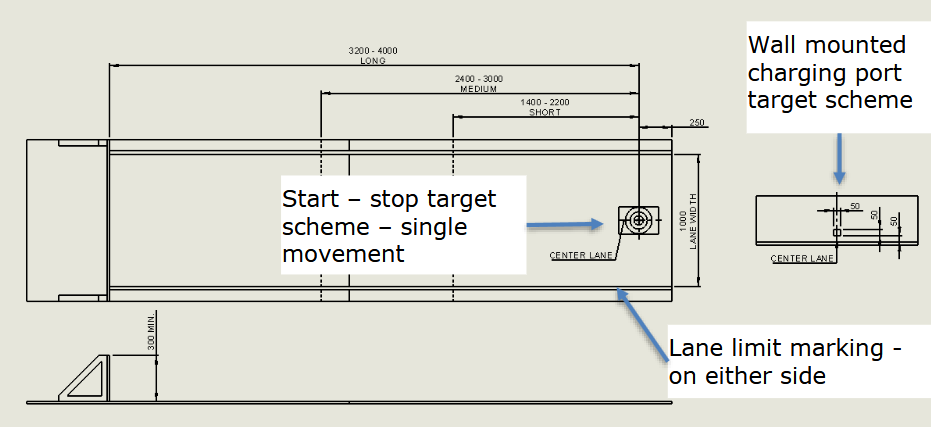
\includegraphics[width=1\textwidth]{extracted_images/image_4_2.png}
\end{center}
\newpage

\section{Product Design Specification}
Safety – The design should not contain any exposed electrical connections and there should be no risk of finger trapping in moveable elements such as the belts and gears.
Size – The device should be able to fit the specified specification.
Aesthetic – Ensure that the design is simple and looks well assembled and appealing.
Cost – The expense of the device should not be able to exceed the given specified budget.
Weight – The weight should be not as heavy since it’ll work more efficiently when it is light.
Durability – The car should be able to withstand pressure and weight so that it isn’t fragile when it hits the wall.

\section{Design Concepts}
\begin{center}
	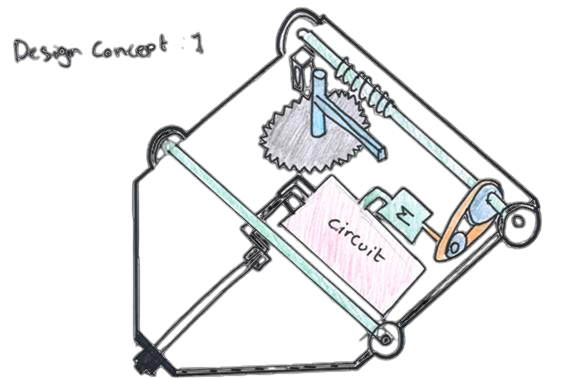
\includegraphics[width=0.7\textwidth]{images/image_6_2-Photoroom.png}
\end{center}\vspace{0.6em}\noindent
This was our first initial concept idea. Its strengths was that it contained little/no refinement however its major weakness was its costliness. It was an accurate model that did however fit the specification, but the major downside was that it contained high manufacturing costs and was complex to build.

\subsection{Evaluation}
A common issue within real world workplaces is manufacturing costs. If the product is too expensive to make it won’t be possible for a worldwide scale of manufacturing due to the costs. Since the product is also too expensive to build, everything will increase such as labour costs, machinery, and time. This will result in a longer time to produce the item and an increase in expenses. The positives of this design is that it does meet the required specifications as it does fit the purpose of its role.\\
\begin{center}
	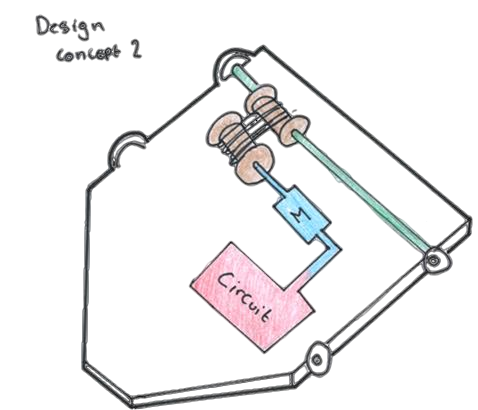
\includegraphics[width=0.7\textwidth]{images/image_7_2-Photoroom.png}
\end{center}\vspace{0.6em}\noindent
This was our second design which was very simple and aesthetically pleasing to look at. Its major strengths was that it was simple to build and small thus resulting in extra space if we needed to exchange or swap parts out. It was a very adaptable design however the major disadvantage to this design was that it is prone easily to breakages.\\[1em]
The negatives of this build is that it is easily prone to breakages which is extremely unreliable. This factor is extremely important since during the testing phase it needs to pass it otherwise the car is not fit to function. If it is prone easily to breakages it will reduce its longevity over time as materials might deteriorate overtime. Since it is also a small design, there will be less space to add any improvements if need be. It is however an aesthetic build since it is versatile and is east to swap parts out if it breaks. The compactness of the build is very efficient too since it enhances the overall aerodynamics of the car and is light since it doesn’t contained compact components.
\begin{center}
	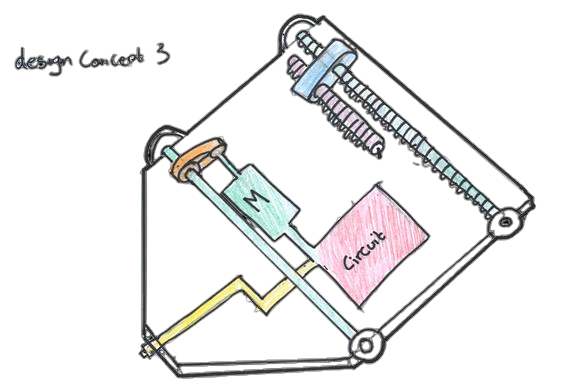
\includegraphics[width=0.7\textwidth]{images/image_8_2-Photoroom.png}
\end{center}\vspace{0.6em}\noindent
This was our final concept idea that again was like our first concept which contained little/no refinement. Its disadvantages was the cost, since it contained many different unique moving parts. It is however, a very durable but complex design but does in fact exceed the budget which is given in the technical specification\\[1em]
The overall budget of this design was very high since there was many different parts needed for it run which increases the manufacturing cost to make it. There was in fact a lack of refinement within this build as there was some inefficiencies within the design itself. It was also very complex which results in a difficult assembly and more chances of errors that be fixed easily if it wasn’t as complex. It was however a durable and strong design which can withstand impact and can perform well.

\section{CAD}

\section{Final design}

\begin{center}
	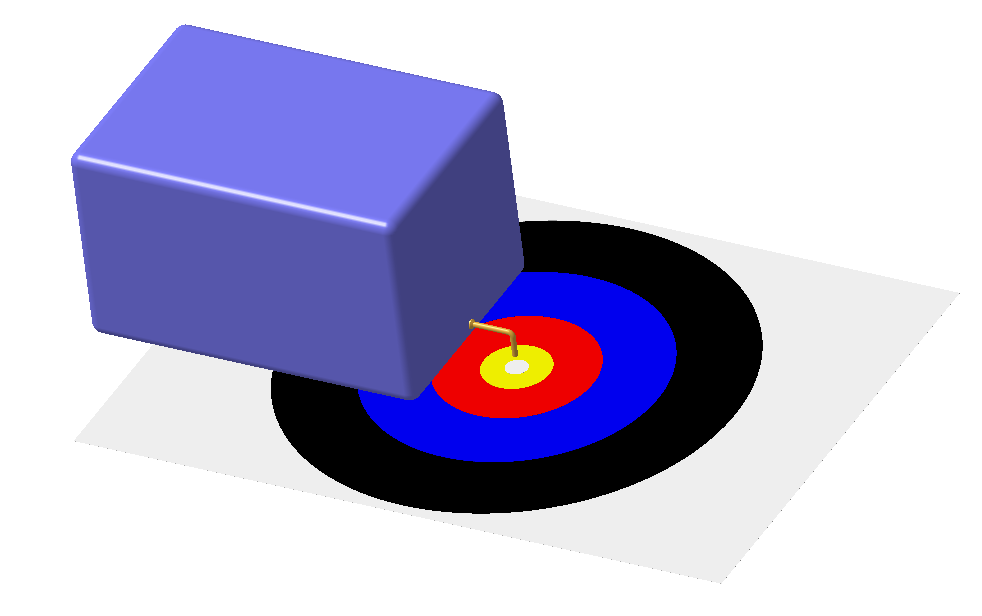
\includegraphics[width=0.7\textwidth]{extracted_images/image_10_2.png}
\end{center}\vspace{0.6em}\noindent
As you can see from the picture provided of the car, you can see that we have fully manufactured a working car that follows all the guidelines and specifications that were required. The main aim of this competition was to create a device that could reach a target there and back under three minutes. The datum pointer should start in the centre of the target and move towards the wall. It should then touch the end of the wall and stay there for 15 seconds then return to the same position as before where the datum pointer started from. The device was safe to use since we ensures that all rules were carefully followed such as electrical connections not being exposed or having the car not fit within the maximum envelope.\\[1em]
As you can see, we received no penalties given since our datum pointer was not too high from the ground. Our front plunger was not larger that it was allowed, and it could realign between the two vertical targets. If the above was not completed it would have resulted in penalties for our team.
\subsection{Size}
The size of envelope is 400x400x400mm which our device was within regulation of. The device should also be able to fit within the envelope throughout the whole competition. We ensured that the datum pointer is in a vertical position and is pointing downwards.
\section{Electronics}

\section{Parts List}
Parts listed for the device are stated below. Every part that was mentioned was used within the final design of the device.
\begin{itemize}[itemsep=-1mm]
	\item Wheels x 4
	\item Lead thread hub x 4
	\item Base x 1
	\item Screw and lead x 1
	\item Plastic tube x 1
	\item Thread screw x 1
	\item Motor x 1
	\item Datum x 1
	\item Belt x 1
\end{itemize}\noindent
Below is a list of the electrical components that were used within the device. Everything mentioned below was used in the final design of the device.
\begin{itemize}[itemsep=-1mm]
	\item 9V Battery
	\item 555 Timer
	\item 10 k$\Omega$ Resistor
	\item 1 k$\Omega$ Resistor
	\item 2.2$\sim\mu$F Capacitor
	\item Red LED
	\item Green LED
	\item 470$\sim\mu$F Capacitor
	\item DPDT Switch
\end{itemize}
These were parts that were essential when building the device. Since we used all components, we did not waste any money, which could have impacted our costs — we could have used the money to purchase better equipment or parts if needed.
\section{Manufacturing process}

\section{BOM (Bill of materials)}
\section{Material list}
\section{References}

\end{document}